\subsection*{Functions Spaces/Finite Elements in Time (FET)}
    As an alternative approach, one can interpret (\ref{eqn:general time-dependent PDE}) on the space-\emph{time} domain $\bfOmega\otimes T$, where $T$ represents a time interval: potentially the timestep $\left(t^{n}, t^{n + 1}\right]$, potentially the whole simulation interval $\left(0, t^{\rm max}\right]$. One then casts into a weak form by testing directly against test functions defined similarly over the whole space-time domain $\bfOmega\otimes T$.
    
    FET transfers the traditional independent choice of RK method to one of a choice of the behavior of the function spaces and Galerkin discretizations in time, in their continuity, order, etc.
    
    A few key points on this technique:
    \begin{itemize}
        \item  For tensor product domains, $\bfOmega\otimes T$, such spaces can often be constructed via the tensor product of spaces on $d$-dimensional $\bfOmega$ and 1-dimensional $T$, without needing to construct new spaces on the entire $(d + 1)$-dimensional domain $\bfOmega\otimes T$.
        \item  The test function spaces need not be identical to the trial function spaces (i.e. a \emph{Petrov}–Galerkin methods) and often won't be for systems with an odd order in time.
        \item  When using a FET interpretation, the intention is often \emph{not} to solve a highly computationally intense, $(d + 1)$-dimensional FE problem on all of $\bfOmega\otimes T$, but to extract a timestepper from the discretization that need only be solved on the $d$-dimensional spatial domain, $\bfOmega$, by exploiting block-triangularity in the stiffness \BA{(Is this the right terminology here?)} matrix. Such block-triangular matrix are derived from well-posed weak forms where the test space has no strongly-imposed initial conditions, such as $*\otimes H^{1}_{+}(T)$ or $*\otimes L^{2}(T)$. \BA{(Check.)} For linear problems, it is in fact often the case that the resultant timesteppers are identical to certain ones that would be derived from a RK-scheme interpretation.
    \end{itemize}
    There are many benefits to a FET interpretation that are often lacking in traditional RK techniques:
    \begin{itemize}
        \item  Crucially, FET provides a weak formulation that often perfectly aligns with the kind of results needed to prove structure-preserving properties.
        \item  FET interpretations inherit much of the useful results and techniques of traditional spatial FEM, including:
        \begin{itemize}
            \item  Finite-element exterior calculus (FEEC).
            \item  Multigrid (at least for non-Petrov–Galerkin schemes).
            \item  Well-studied interpolation and projection error estimates.
            \item  Language for the analysis and interpretation of non-confoming schemes.
            \item  Agency over bases for the time discretization with good orthogonality properties. \BA{(FDM- I want to make a remark on this later.)}
            \item  Easy extension to high order
        \end{itemize}
        \item  Solutions provided by FET are meaningful at all times. \BA{(This is important for me.)}
        \item  FET is the perfect language for solving problems that are already posed on a space-time domain, such as:
        \begin{itemize}
            \item  Searching for periodic solutions. \BA{(I need to do a good note about this somewhere- about how we solve for time periods for periodic problems, since this is something I really want to consider.)}
            \item  Problems with moving boundaries, where the space-time domain can \emph{not} be written in the tensor-product form $\bfOmega\otimes T$.
        \end{itemize}
    \end{itemize}
    \line
    \begin{example}[CG-DG-in-time discretization for the heat equation]
        Consider the heat equation (\ref{eqn:heat equation}) on $\bfOmega\otimes T$ for $T  =  \left(0, t^{\rm max}\right]$, with homogeneous Dirichlet/Neumann boundary conditions, such that in the strong form, the dissipation equation (\ref{eqn:heat equation dissipation}) holds. Suppose further the initial conditions (ICs) at $t  =  0$, $u  =  \widehat{u}_{0}|_{t = 0}$ hold.
        
        To cast into a chosen weak form in time, define:
        \begin{itemize}
            \item  A test space $\calU$, with $\calU_{-}  :=  \{u  \in  \calU  : 
         u|_{t = 0}  =  0\}$
            \item  A trial space $\calV$
        \end{itemize}
        supported on $\bfOmega\otimes T$. One seeks $u_{-}  \in  \calU_{-}$ such that $\forall  v  \in  \calV$,
        \begin{equation}\label{eqn:heat equation weak form}
            \langle v, \partial_{t}u\rangle_{\bfOmega\otimes T}  =   - \frac{1}{\rmPe}\langle\nabla v, \nabla u\rangle_{\bfOmega\otimes T},
        \end{equation}
        where, to incorporate the ICs, $u$ is $u_{-}$ with a lifting of the ICs, $u  :=  u_{0} + u_{-}$, where in turn $u_{0}  \in  \calU$ is an extension of the ICs to be supported on $\bfOmega\otimes T$.
        
        To create an order-$s$ CG-DG FET timestepper, define:
        \begin{align}
            \bbU^{h}  :=  \widehat{\calU}(\bfOmega)\otimes\bbP^{s}\left(T^{h}\right)  <  \calU,  &&
            \bbV^{h}  :=  \widehat{\calV}(\bfOmega)\otimes\bbDP^{s - 1}\left(T^{h}\right)  <  \calV,
        \end{align}
        where $T^{h}$ is a mesh of intervals on $T$, at timesteps $0$, $t^{1}$, $t^{2}$, $\cdots$, with $\bbU^{h}_{-}$ defined analogously to $\calU_{-}$. Mapping $\calU_{-}  \mapsto  \bbU^{h}_{-}$, $\calV_{-}  \mapsto  \bbV^{h}_{-}$ in (\ref{eqn:heat equation weak form}) invokes the Petrov–Galerkin projection. Denote bases for these FE spaces:
        \begin{align}
            (\phi_{j})_{j}     \text{ for }  \bbP^{s}\left(T^{h}\right),         &&
            (\varphi_{i})_{i}  \text{ for }  \bbDP^{s - 1}\left(T^{h}\right).
        \end{align}
        $u^{h}  \in  \bbU^{h}$, $v^{h}  \in  \bbV^{h}$ can be expressed in terms of these bases as:
        \begin{align}
            u^{h}(\bfx; t)  =  \sum_{j}\widehat{u}_{j}(\bfx)\phi_{j}(t),  &&
            v^{h}(\bfx; t)  =  \sum_{i}\widehat{v}_{i}(\bfx)\varphi_{i}(t)
        \end{align}
        for $\left(\widehat{u}_{j}\right)_{j}$ in $\widehat{\calU}$, $\left(\widehat{v}_{i}\right)_{i}$ in $\widehat{\calV}$. The Petrov–Galerkin-projected weak form then states that, $\forall  (v_{i})_{i}$:
        \begin{align}
            \left\langle\sum_{i}\widehat{v}_{i}\varphi_{i}, \partial_{t}\left[\sum_{j}\widehat{u}_{j}\phi_{j}\right]\right\rangle_{\bfOmega\otimes T^{h}}  &=  - \frac{1}{\rmPe}\left\langle\nabla\left[\sum_{i}\widehat{v}_{i}\varphi_{i}\right], \nabla\left[\sum_{j}\widehat{u}_{j}\phi_{j}\right]\right\rangle_{\bfOmega\otimes T^{h}}  \\
            \sum_{i, j}\left\langle\widehat{v}_{i}, \widehat{u}_{j}\right\rangle_{\bfOmega}\langle\varphi_{i}, \partial_{t}\phi_{j}\rangle_{T^{h}}  &=  - \frac{1}{\rmPe}\sum_{i, j}\left\langle\nabla\widehat{v}_{i}, \nabla\widehat{u}_{j}\right\rangle_{\bfOmega}\langle\varphi_{i}, \phi_{j}\rangle_{T^{h}}
        \end{align}
        Denoting the vectors $\widehat{\bfu}  :=  \left(\widehat{u}_{j}\right)_{j}$, $\widehat{\bfv}  :=  \left(\widehat{v}_{i}\right)_{i}$, and mass and stiffness bilinear operators $\calM\left[\widehat{v}, \widehat{u}\right]  :=  \left\langle\widehat{v}, \widehat{u}\right\rangle_{\bfOmega}$, $\calK\left[\widehat{v}, \widehat{u}\right]  :=  \left\langle\nabla\widehat{v}, \nabla\widehat{u}\right\rangle_{\bfOmega}$ respectively, this takes the matrix form
        \begin{align}
            \widehat{\bfv}^{\rmT}(\langle\varphi_{i}, \partial_{t}\phi_{j}\rangle_{T^{h}}\calM)_{ij}\widehat{\bfu}  =  - \frac{1}{\rmPe}\widehat{\bfv}^{\rmT}(\langle\varphi_{i}, \phi_{j}\rangle_{T^{h}}\calK)_{ij}\widehat{\bfu},  \\
            \widehat{\bfv}^{\rmT}\left(\langle\varphi_{i}, \partial_{t}\phi_{j}\rangle_{T^{h}}\calM + \frac{1}{\rmPe}\langle\varphi_{i}, \phi_{j}\rangle_{T^{h}}\calK\widehat{\bfu}\right)_{ij}\widehat{\bfu}  =  0
        \end{align}
        
        Regarding the sparsity of this matrix, with appropriate ordering of the bases $(\phi_{i})_{i}$, $(\varphi_{i})_{i}$, the matrices $(\langle\varphi_{j}, \partial_{t}\phi_{l}\rangle_{T^{h}})_{j}^{l}$, $(\langle\varphi_{j}, \phi_{l}\rangle_{T^{h}})_{j}^{l}$ take the general form
        \begin{equation}\label{eqn:timestepper matrices}
            \left(\begin{array}{ c : c c : c c : c c }
                \pm\bfb  &  \bfA    &  \bfb     &  0       &  0        &  \cdots   &  0        \\
                \hdashline
                0        &  0       &  \pm\bfb  &  \bfA    &  \bfb     &  \cdots   &  0        \\
                \hdashline
                0        &  0       &  0        &  0       &  \pm\bfb  &  \cdots   &  0        \\
                \hdashline
                \vdots   &  \vdots  &  \vdots   &  \vdots  &  \vdots   &  \ddots   &  \vdots   \\
                \hdashline
                0        &  0       &  0        &  0       &  0        &  \cdots   &  \bfb     \\
            \end{array}\right)
        \end{equation}
        for some $\bfA  \in  \bbR^{q\times (q - 1)}$, $\bfb  \in  \bbR^{q}$ in either case, dependent on the choice of bases. (See Figure \ref{fig:timestepper matrices}) \BA{(Capitalization on ``Figure''?)}

        \begin{figure}[!ht]
            \centering
            \begin{subfigure}{0.5\textwidth}
                \centering
                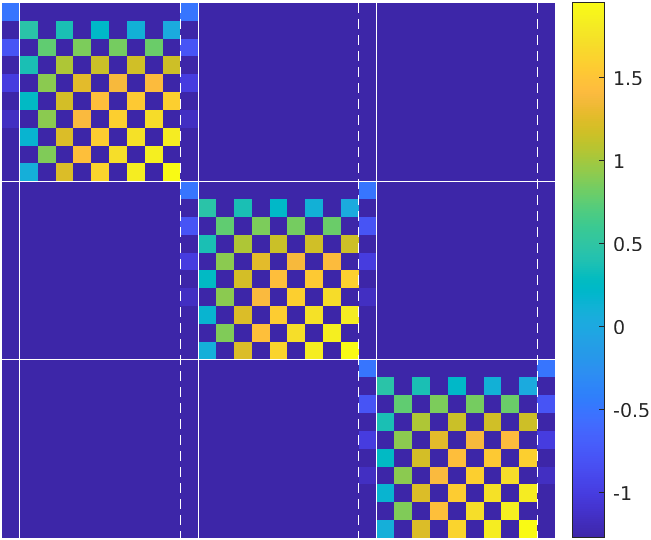
\includegraphics[width = 0.9\textwidth]{9 - finite elements in time/images/matrix 1.png}
                \caption{$(\langle\varphi_{j}, \partial_{t}\phi_{l}\rangle_{T^{h}})_{j}^{l}$}
            \end{subfigure}%
            \begin{subfigure}{0.5\textwidth}
                \centering
                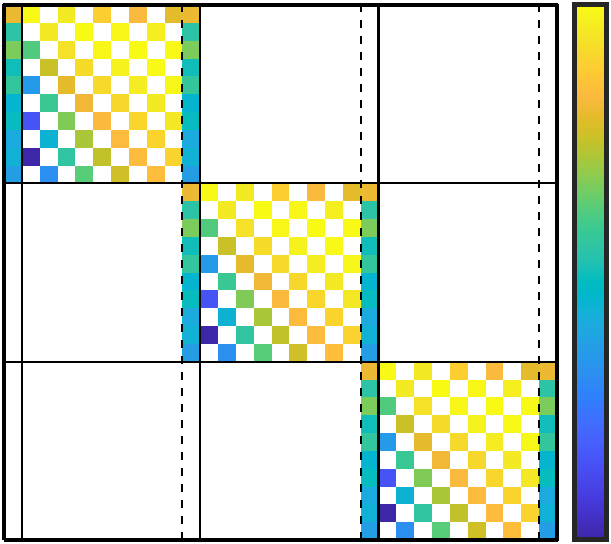
\includegraphics[width = 0.9\textwidth]{9 - finite elements in time/images/matrix 2.png}
                \caption{$(\langle\varphi_{j}, \phi_{l}\rangle_{T^{h}})_{j}^{l}$}
            \end{subfigure}
            \caption{Sparsity plots for the two timestepping matrices when $q = 10$ on 3 (equal) intervals, under simple normalised polynomial bases. \\ Color indicates $\log(|*|)$ for the matrix entries. Black lines indicate block structure from (\ref{eqn:timestepper matrices}), while solid black lines highlight the lower-block-triangular structure after elimination of first column.}
            \label{fig:timestepper matrices}
        \end{figure}

        With strongly-imposed initial conditions on $\bbU^{h}$, the first column of this matrix is eliminated, leaving a lower-block-triangular matrix of size-$p$ blocks, as indicated by the dashed lines in (\ref{eqn:timestepper matrices}). Applying block forward substitution to solve this block triangular problem is perfectly analogous to using a traditional timestepper.

        Denoting, $\bfu_{l}  :=  (u_{kl})_{k}$, on the $n$-th timestep, the resultant linear problem takes the form:
        \begin{equation}
            \left[(\langle\varphi_{nq + j}, \partial_{t}\phi_{nq + l}\rangle_{T^{h}})_{j = 1, \cdots, q}^{l = 0, \cdots, q}\otimes\bfM + \kappa(\langle\varphi_{nq + j}, \phi_{nq + l}\rangle_{T^{h}})_{j = 1, \cdots, q}^{l = 0, \cdots, q}\otimes\bfK\right](\bfu_{nq + l})_{l = 0, \cdots, q}  =  \bfzero
        \end{equation}
        \begin{multline}
            \left[(\langle\varphi_{nq + j}, \partial_{t}\phi_{nq + l}\rangle_{T^{h}})_{j = 1, \cdots, q}^{l = 1, \cdots, q}\otimes\bfM + \kappa(\langle\varphi_{nq + j}, \phi_{nq + l}\rangle_{T^{h}})_{j = 1, \cdots, q}^{l = 1, \cdots, q}\otimes\bfK\right](\bfu_{nq + l})_{l = 1, \cdots, q}  \\
            =  - [(\langle\varphi_{nq + j}, \partial_{t}\phi_{nq}\rangle_{T^{h}})_{j = 1, \cdots, q}\otimes\bfM + \kappa(\langle\varphi_{nq + j}, \phi_{nq}\rangle_{T^{h}})_{j = 1, \cdots, q}\otimes\bfK]\bfu_{nq}
        \end{multline}
        which can be solved iteratively for each $\bfu_{(n + 1)q}$ at each new timestep.

        In the case of $q = 1$—the lowest-order method—with time intervals of length $\delta t$, this takes the form
        \begin{equation}
            \left[\bfM + \kappa\frac{\delta t}{2}\bfK\right]\bfu_{n + 1}  =  \left[\bfM - \kappa\frac{\delta t}{2}\bfK\right]\bfu_{n},
        \end{equation}
        which, by rearranging, can be seen to be equivalent to the traditional implicit midpoint method,
        \begin{equation}
            \bfM\left[\frac{1}{\delta t}(\bfu_{n + 1} - \bfu_{n})\right]  =  - \kappa\bfK\left[\frac{1}{2}(\bfu_{n + 1} + \bfu_{n})\right],
        \end{equation}
        or, in weak formulation,
        \begin{equation}
            \left\langle v^{h}_{n + 1}, \frac{1}{\delta t}\left(u^{h}_{n + 1} - u^{h}_{n}\right)\right\rangle_{\bfOmega^{h}}  =  - \left\langle\nabla v^{h}_{n + 1}, \frac{1}{2}\nabla\left(u^{h}_{n + 1} + u^{h}_{n}\right)\right\rangle_{\bfOmega^{h}}.
        \end{equation}

        \BA{Would be nice to restructure this example to generally talk more in the weak formulations than with all these mass/stiffness matrices that aren't necessarily relevant to understanding how FEs in time give rise to timesteppers.}
    \end{example}

    \line
    
    \BA{Should go through and add correct punctuation to my equations.}


    